\section{Historie}
Alle \currentauthor{David Piper} in dieser Ausarbeitung vorgestellte Algorithmen zur Konstruktion des Suffix-Arrays lassen sich in drei Gruppen einteilen, welche die grundlegenden Sortierverfahren beschreiben. \par
Die erste Gruppe bilden die sogenannten \textit{prefix doubler}, zu welcher die Algorithmen Prefix Doubling und qSufSort gehören.
Wie in Abschnitt \ref{sec:ansatz:doubler} beschrieben wird, sortieren diese die Präfixe der Suffixe und können durch geschickte Ideen die Sortierung beschleunigen, indem die Anzahl der betrachteten Präfixe in jedem Schritt verdoppelt wird. 
Dabei setzte der SACA Prefix Doubling, welcher der Vorgänger des in dieser Ausarbeitung behandelten gleichnamigen SACAs ist, die Grundlagen für diese Kategorie.
Darauf aufbauend ermöglichte qSufSort eine effizientere Konstruktion des Suffix-Arrays. 
Neben diesen beiden Algorithmen gehört auch der Algorithmus BPR teilweise in diese Gruppe, nutzt jedoch ebenfalls Ideen eines zweiten Verfahrens, dem \textit{Induzieren}. \par

Zur Gruppe der Induzierer gehören auch die Algorithmen Deep-Shallow, DivSufSort, mSufSort, SAIS und GSACA.
Sie sortieren Suffixe anhand bereits zuvor sortierter Suffixe.
Dieses Konzept wird näher im Absatz \ref{section:induzierer} beschrieben.
Deep-Shallow war von den hier behandelten Algorithmen der erste, welcher dieses Verfahren nutzte.
Von ihm wurde der Algorithmus DivSufSort inspiriert, dessen Implementierungsdetails teilweise in die Entwicklung von SAIS eingingen.
SAIS führte Ideen ein, welche auch von GSACA aufgegriffen wurden.
Hingegen bildet mSufSort eine neu Vererbungslinie und baut auf keinem der anderen SACAs auf.
Auch nzSufSort und SACA-K gehörten zu dieser Gruppe, kombinieren das induzierte Sortieren jedoch mit dem Konzept der letzten Gruppe. \par

Diese nutzt Rekursion, um kleinere Teilmengen von Zeichen zu Sortieren, welche dann zum finalen Suffix-Array zusammengesetzt werden.
Zusätzlich zu nzSufSort und SACA-K wird dieses Sortierverfahren auch von den SACAs DC3 und SADS verwenden. 
Der erste Algorithmus, welcher rekursiv arbeitete, um ein Suffix-Array zu erstellen, war DC3.
Der Algorithmus nzSufSort wurde unter anderem von DC3 inspieriert, und greift manche der enthaltenen Ideen auf.
Auch die beiden Suffix-Array-Konstruktionsalgorithmen SAIS und SADS gehörten zu dieser Gruppe.
SACA-K, welcher sowohl induziert als auch rekursiv arbeitet, ist eine Weiterentwicklung der Ideen von SAIS und SADS und stellt dabei sowohl eine Verbesserung der Laufzeit als auch des Speicherverbrauchs dar. \par

\begin{figure}[H]
	\centering
	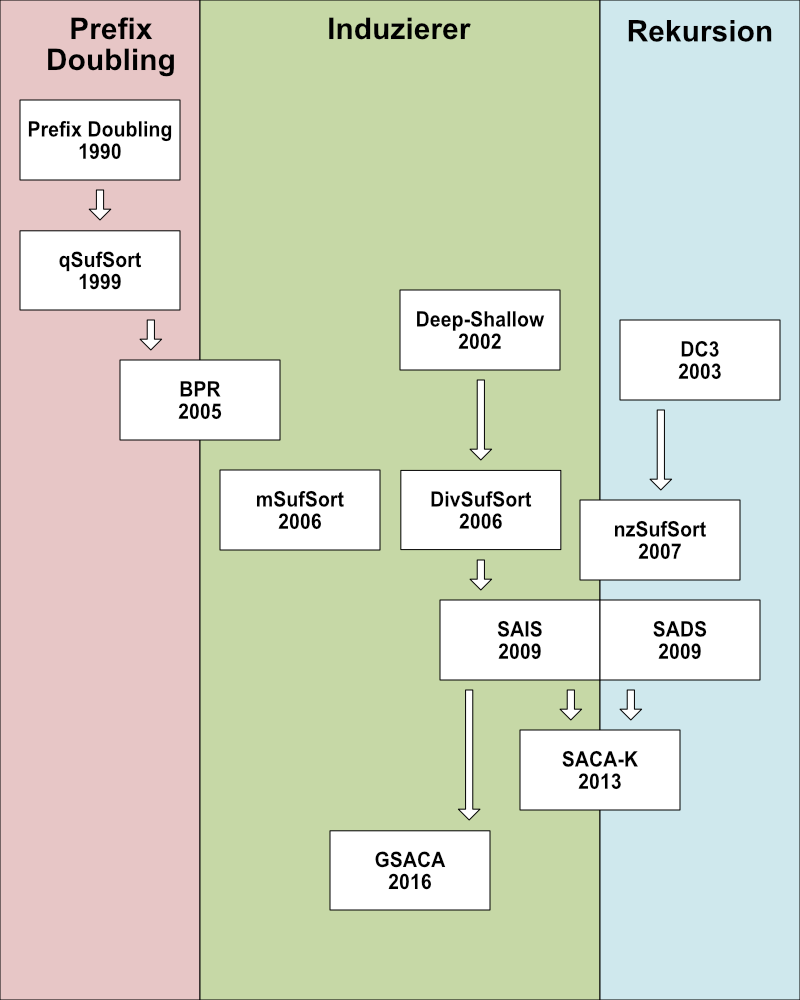
\includegraphics[width=\linewidth]{kapitel/5_saca_uebersicht/history/history3}
	\caption{Geschichtliche Entwicklung von SACAs, die in dieser Ausarbeitung betrachtet werden.}
	\label{fig_banane_1_2}
\end{figure}
